\documentclass{article}
\usepackage{graphicx} % Required for inserting images

\documentclass[a4paper, 12pt]{article}%тип документа
\usepackage{xcolor}
%отступы
\usepackage[left=2cm,right=2cm,top=2cm,bottom=3cm,bindingoffset=0cm]{geometry}
\usepackage[pdftex]{lscape}
%Русский язык
\usepackage[T2A]{fontenc} %кодировка
\usepackage[utf8]{inputenc} %кодировка исходного кода
\usepackage[english,russian]{babel} %локализация и переносы
\usepackage{multirow}
%Вставка картинок
\usepackage{wrapfig}
\usepackage{graphicx}
\graphicspath{{Images/}}
\DeclareGraphicsExtensions{.pdf,.png,.jpg}

%Математика
\usepackage{amsmath, amsfonts, amssymb, amsthm, mathtools}

%Заголовокhttps://www.overleaf.com/project/6507f5a4176b25bf05722230

\begin{document}

\begin{titlepage}
	\begin{center}
		{\large МОСКОВСКИЙ ФИЗИКО-ТЕХНИЧЕСКИЙ ИНСТИТУТ (НАЦИОНАЛЬНЫЙ ИССЛЕДОВАТЕЛЬСКИЙ УНИВЕРСИТЕТ)}
	\end{center}
	\begin{center}
		{\large Физтех-школа биологической и медицинской физики}
	\end{center} 
	
	
	\vspace{4.5cm}
	{\huge
		\begin{center}
			{\bf Отчёт о выполнении лабораторной работы}\\
			Основы MALDI-TOF масс-спектрометрии
		\end{center}
	}
	\vspace{4.5cm}
	\begin{flushright}
		{\LARGE Авторы:\\ Акимов Максим \\ Кондратюк Наталья \\ 
			\vspace{0.5cm}
			Б06-206}
	\end{flushright}
	\vspace{4cm}
	\begin{center}
		Долгопрудный 
       \\20 января 2025 года
	\end{center}
 
\end{titlepage}

\newpage 
\section{Аннотация}
\paragraph*{Цель работы:}  Применение метода MALDI-TOF масс-спектрометрии для изучения пептидной смеси.
\paragraph*{Задачи:}
\begin{itemize}
    \item Получение масс-спектра смеси пептидов с матрицей HCCA без и с использованием рефлектрона;
    \item Идентификация пиков на масс-спектре и определение состава пептидной смеси;
    \item Определение зависимости основных аналитических характеристик масс-спектрометра от экспериментальных параметров: мощности лазера, уровня подавления матрицы, времени включения ускоряющего потенциала
\end{itemize}
\section{Введение}
\subsection{Основные понятия и процессы}\;
\par Масс-спектрометрия – физический метод исследования вещества, основанный на детектировании отношения массы к заряду (m/z) ионизированных молекул и атомов. Результат измерения на масс-спектрометре количества зарегистрированных детектором ионов с определенным отношением массы к заряду называется масс-спектром.
В общем случае можно выделить следующие функциональные блоки и системы масс-спектрометра: система ввода пробы в масс-спектрометр, источник ионизации, масс-анализатор, вакуумная система, детектор и система регистрации и обработки сигналов. Под системой ввода пробы в
масс-спектрометр (конкретно – в источник ионизации) подразумевается комплекс устройств, служащих для ввода пробы в область ионного источника, в том числе разнообразные интерфейсы атмосфера-высокий вакуум и отдельно подключаемые устройства (например, газовый
баллон или хроматограф). Также имеются системы управления и питания устройств масс-спектрометра и системы ионной (электронной) оптики.

Несмотря на достаточно активные исследования, общепринятого понимания всех физических и химических процессов, происходящих при ионизации методом MALDI, до сих пор не существует. Большое число предложенных возможных моделей сходится только в одном: процесс ионизации в MALDI состоит из двух стадий.


\textbf{Первая стадия} – образование первичных свободных ионов из молекул матрицы. Описывает процесс фазового перехода «твердое тело–газ». При высоких интенсивностях лазерного излучения он может быть охарактеризован как абляция. Это процесс «взрывного» испарения твердого тела: образец перегревается и происходит подповерхностная нуклеация (зародышеобразование), вызывающая «фазовый взрыв». Над поверхностью образца возникает область высокого локального давления – так называемый «факел» (plume – факел, шлейф). На этой стадии как твердое тело, так и газ могут содержать нейтральные и ионизованные кластеры молекул матрицы и аналита. Продолжительность первого этапа примерно соответствует продолжительности импульса лазера и практически совпадает со временем жизни возбужденных состояний матрицы. Данная стадия носит название \textbf{первичная ионизация}.

\textbf{Вторая стадия} – формирование ионов анализируемого вещества в газовой фазе в результате взаимодействия ионов матрицы и нейтральных молекул анализируемого вещества (ион-молекулярные процессы). Этой стадии соответствует период адиабатического расширения образовавшихся после лазерного импульса продуктов (длительность стадии порядка 10 мкс). Это \textbf{вторичная ионизация}.

\subsection{MALDI-TOF масс-спектрометрия}\;
\par Для анализа ионов и определения значений m/z в масс-спектрометрии применяются различные типы масс-анализаторов, среди которых наиболее распространенными являются времяпролетные, квадрупольные, ионные ловушки. В масс-спектрометре с источником MALDI чаще всего применяются времяпролетные (Time of Flight или сокращенно TOF) масс-анализаторы.
Упрощенная схема MALDI-TOF масс-спектрометра состоит из короткой области I в источнике ионов c высоким значением напряженности E электрического поля и более длинной бесполевой области II – области дрейфа. Типичная длина указанных областей: $s = 1 \; \text{см},\; D = 1 \; \text{м}$. 

В общем случае, время пролёта иона к детектору вычисляется, как

$$
t = \sqrt{m/z}\cdot const + t_0
$$
\begin{figure}[h!]
        \centering
        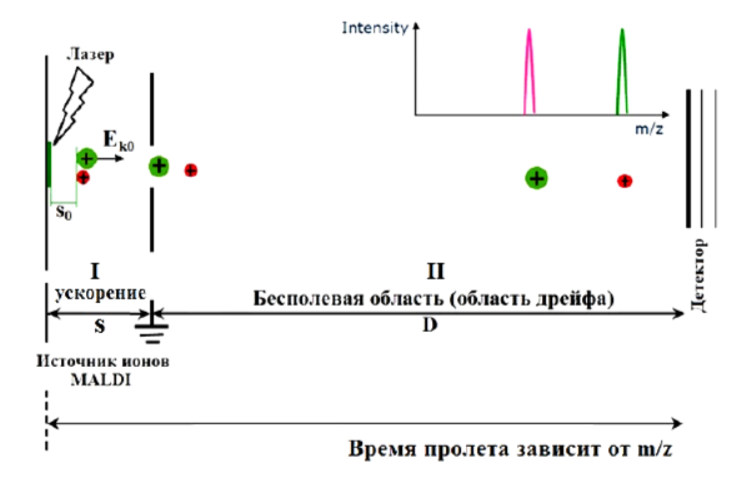
\includegraphics[scale=0.4]{Images/2025-01-18_23-30-59.png}
        \caption{Принцип действия масс-спектрометра с времяпролётным масс-анализатором}
\end{figure}

\subsection{Метод импульсной экстракции ионов, PIE}\;
\par Для устранения теплового разброса ионов A+ по начальным
кинетическим энергиям и повышения разрешающей способности TOF масс-анализаторов применяется метод временной задержки фокусировки(Time-Lag Focusing) или, что то же самое, метод импульсной экстракции
ионов (Pulsed Ion Extraction, PIE). В процесс PIE вовлечены три компонента источника ионов, а именно мишень (IS1), на которую наносят образец, пластина вторичного напряжения (IS2), которая представляет собой электрод, приподнятый на несколько миллиметров от образца, и следующий заземленный ускоряющий электрод. 

Метод PIE работает следующим образом. На первом этапе мишень IS1
с нанесенным анализируемым образцом всегда имеет потенциал $\phi_1$. Экстрагирующая пластина IS2 подсоединена к тому же потенциалу $\phi_1$. Таким же образом, анализируемое вещество не подвергается воздействию каких-либо внешних эффектов до удара лазерного луча, с которого начинается этап 2 На этом этапе в «факеле» MALDI происходит ионизация анализируемого вещества и тепловой дрейф образующихся ионов A+ от IS1 к IS2
(по-прежнему $\phi_1 = \phi_2$, и выталкивающее электрическое поле отсутствует). Из-за теплового разброса не все ионы обладают одинаковой начальной скоростью. Некоторые «быстрые» пролетают дальше, чем другие «медленные». На третьем этапе после некоторого времени задержки tdelay (от момента начала импульса лазера) потенциал IS2 импульсно снижается от величины $\phi_1$ до $\phi_2$, создавая электрическое поле, которое заставляет все заряженные частицы двигаться по направлению к IS2.
В результате ионы с меньшей начальной скоростью оказываются в
точке с большим потенциалом, а ионы с большей начальной скоростью – в точке с меньшим потенциалом электрического поля. При правильном подборе времени задержки и величины электрического импульса (амплитуды и длительности) ионы заданной массы с различными начальными скоростями достигнут детектора одновременно. 

\begin{figure}[h!]
        \centering
        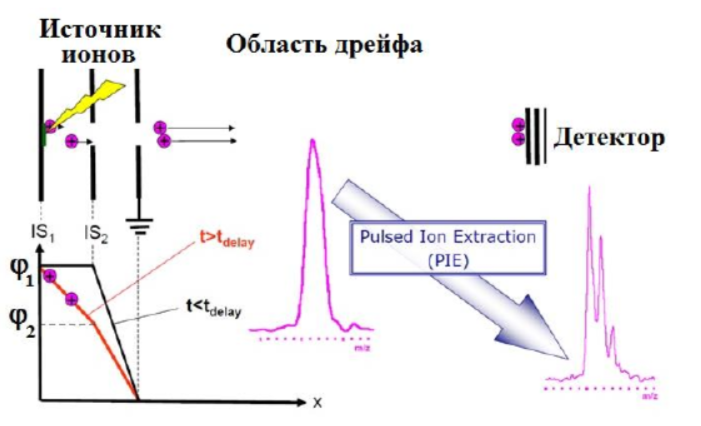
\includegraphics[scale=0.4]{Images/2025-01-18_23-43-26.png}
        \caption{Принцип работы PIE}
\end{figure}
\newpage
\subsection{Рефлектрон}\;
\par Для дальнейшей компенсации различия в энергиях ионов и улучшения разрешения необходимо использовать рефлектрон (ионное зер-
кало).
Система ultraflex и другие времяпролетные масс-спектрометры серии
«flex» используют двухступенчатый бессеточный рефлектрон с электро-
статическими линзами. В данном рефлектроне при помощи электростатического поля ионы отражаются под небольшим углом в направлении детектора рефлектрона. Ионы с большей кинетической энергией из группы ионов с одной массой проникают глубже внутрь отражающего поля рефлектрона, тем самым затрачивая больше времени на замедление и последующее ускорение. Достигая ионного зеркала первыми, они последними покидают его и догоняют более медленные ионы в фокальной плоскости, в которой располагается детектор. Такой принцип приводит к значительному увеличению разрешения времяпролетных приборов с рефлектроном по сравнению со спектрометрами без него и одновременно увеличивает точность определения масс.
\section{Экспериментальная установка}
Тандемный времяпролетный масс-спектрометр «ULTRAFLEX MALDI TOF/TOF» создан для автоматизированных высокопроизводительных анализов методами МС и МС/МС (тандемная масс-спектрометрия) белков и пептидов. В настоящей работе используется только метод измерений МС.
Прибор может работать в одном из двух режимов регистрации ионов: положительных либо отрицательных ионов (в работе используется «положительный» режим). Диапазон работы масс-анализатора составляет от 20 до 260000 Да. На рисунке изображена схема данного масс-спектрометра и показан принцип его работы. Изображены источник ионов с помещенной в него мишенью, область дрейфа, детектор, работающий в т.н. «линейном режиме» (без использования рефлектрона), рефлектрон и детектор, работающий в паре с ним.
\begin{figure}[h!]
        \centering
        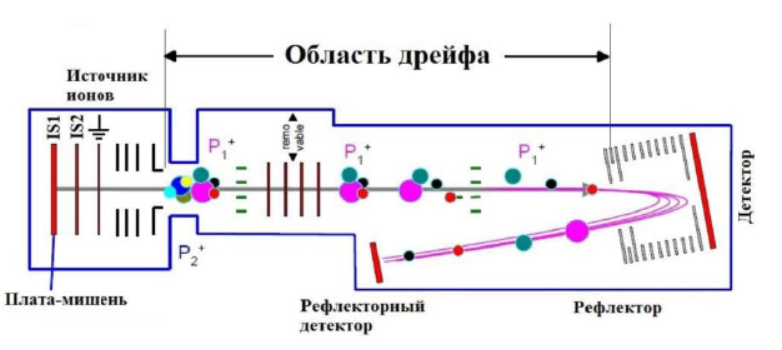
\includegraphics[scale=0.7]{Images/Снимок экрана 2025-01-18 232036.png}
        \caption{ Принцип действия масс-спектрометра «ULTRAFLEX MALDI TOF/TOF»}
\end{figure}
Вакуумная система «ULTRAFLEX MALDI TOF/TOF». Условия высокого вакуума, требуемые для проведения измерений (давление около $6 \cdot 10^{-7}$ торр и ниже), создаются при помощи турбомолекулярных насосов в источнике ионов и в трубке, по которой пролетают ионы. Для начала работы турбомолекулярных насосов необходимо наличие низкого вакуума, создаваемого форвакуумным насосом.

Лазерная система состоит из импульсного УФ лазера ($N_2$-лазер с длиной волны 337 нм с энергией в импульсе 100 мкДж и длительностью импульса от десятых до единиц наносекунд; диаметр луча примерно 1-10 мкм), аттенюатора, обеспечивающего правильную регулировку
интегральной плотности потока лазерного излучения, системы линз, фокусирующих лазерный пучок, и системы зеркал, направляющих пучок в источник ионов, на мишень.
Источник ионов – часть масс-спектрометра, в которой ионы образуются в результате лазерной десорбции/абляции. Он состоит из трех основных частей: x-y-Платформа,
шлюзовая система и ионно-оптическая система.
x-y-Платформа обеспечивает перенос мишени с нанесенным на нее образцом внутрь источника ионов (и обратно) и перемещения мишени в координатах x-y. Образец наносится в специальные расположенные на мишени углубления — «ячейки» мишени, размеченные буквами A, B, ..., P по оси Y и цифрами 1, 2, ..., 24 – по оси Х.
Шлюзовая система используется при загрузке и выгрузке мишени. Работает подобно буферу, разделяющему область при атмосферном давлении и область низкого вакуума посредством клапана. Область высокого вакуума также отделена от низкого вакуума соответствующим клапаном.
Система ионной оптики служит для формирования, фокусировки и отклонения ионного луча. Она состоит из положительно или отрицательно заряженной мишени,
пластины вторичного напряжения и заземленного ускоряющего электрода.
 \begin{figure}[h!]
        \centering
        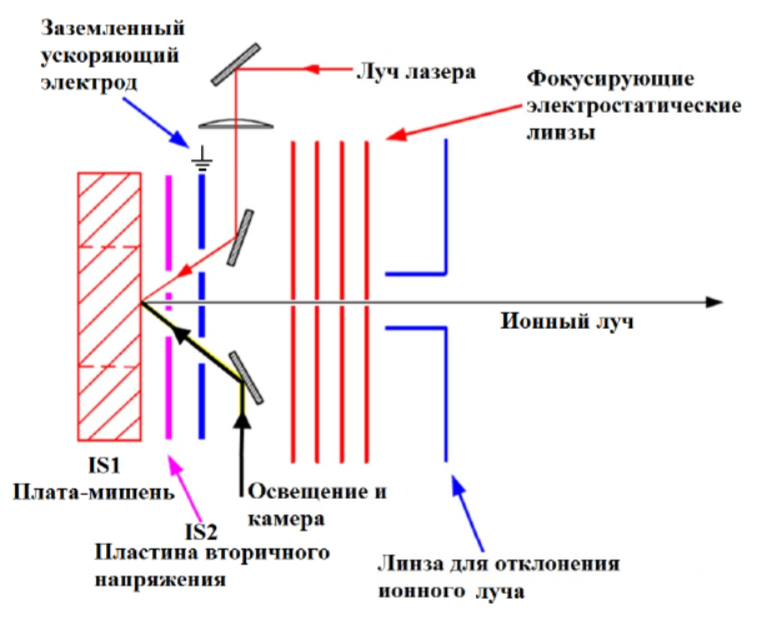
\includegraphics[scale=0.4]{Images/2025-01-18_23-20-44.png}
        \caption{Схема источника ионов, используемого в MALDI-TOF масс-спектрометре}
\end{figure}

\section{Результаты и обсуждение}
\subsection{Исследование масс-спектрометрии без рефлектрона}
\subsubsection{Идентификация масс-спектров}\;
\par Установим режим измерения на $"Default\_linear"$, подразумевающий измерения на установке без использования рефлектрона. Измерения будем проводить на лунке B22. Для идентификации масс-спектров используем максимальную мощность лазера ($P = 100 \%$). Полученный спектр продемонстрирован на Рис.\ref{Идентификация}.
\begin{figure}[h!]
\centering
    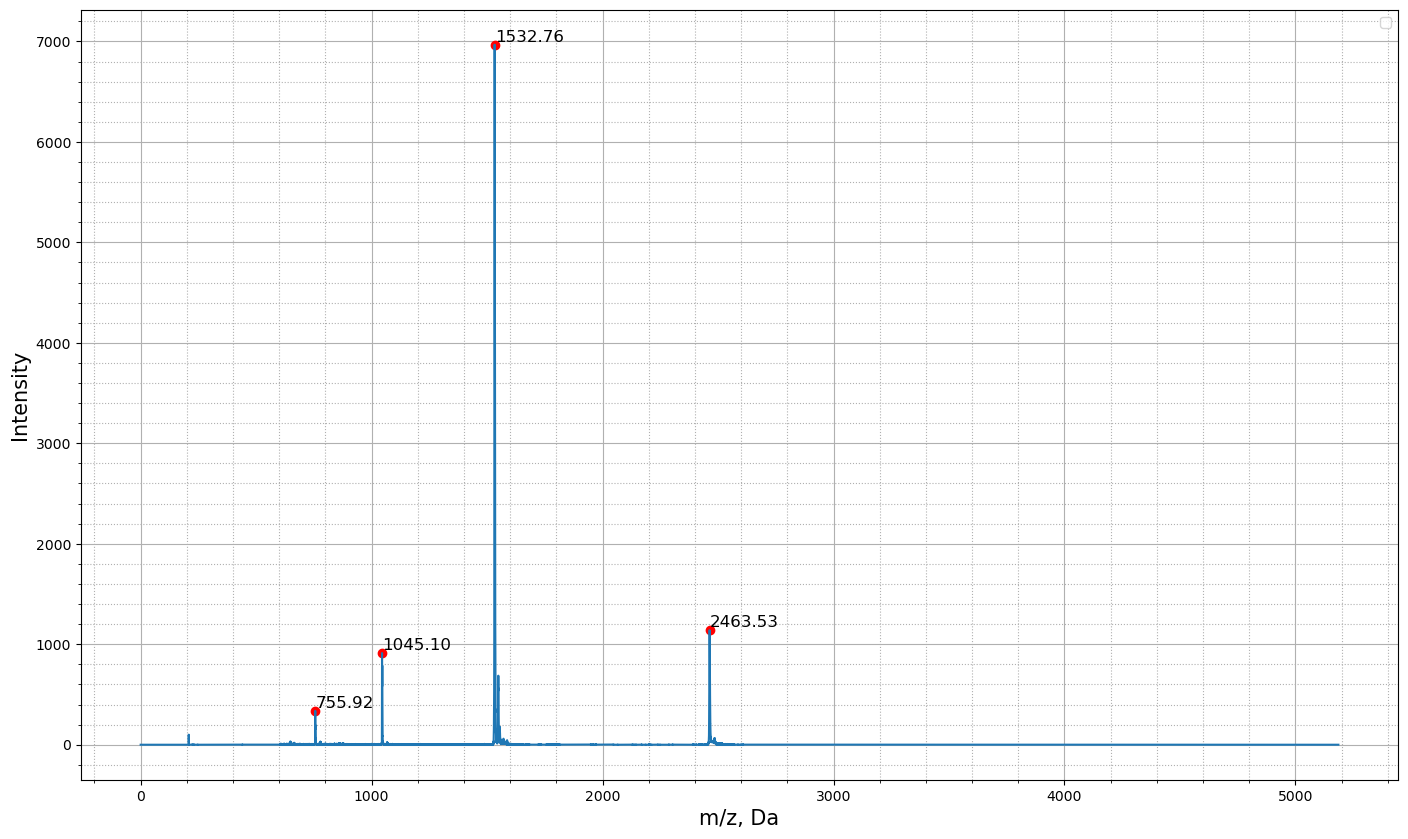
\includegraphics[width=\linewidth]{Images/linear_peaks.png}
    \caption{Масс-спектр лунки B22; без рефлектрона; $P = 100 \%$}
    \label{Идентификация}
\end{figure}

Исходя из представленного изображения (и списка возможных белков в методичке), можно сделать вывод (с погрешностью в $1\; Da$), что в лунке содержатся следующие белки или их фрагменты:
\begin{itemize}
    \item $756\pm1 \; Da$ - Bradykinin (1–7)
    \item $1046\pm1 \; Da$ - Angiotensin II
    \item $1533 \pm 1 \; Da$ - P14R
    \item $2464 \pm 1 \; Da$ - ACTH (18–39)
\end{itemize}

В дальнейшей работе показатели для этих пиков будут сравниваться при изменении параметров масс-спектрометра. 

\subsubsection{Определение зависимости аналитических характеристик метода от мощности лазера}\;
\par В качестве характеристик метода предлагаются:
\begin{itemize}
    \item Отношение сигнал/шум ($S/N = \frac{Peak \; Intensity}{Noise}$)
    \item Разрешение ($Resolution = \frac{m/z}{\Delta(m/z)}$)
\end{itemize}

Для начала будем менять мощность лазера с $10 \; \%$ до $100 \; \%$ и измерять необходимые нам параметры. В качестве визуальной иллюстрации наложим все спектры друг на друга и проследим общую зависимость Рис.\ref{Мощность}.
\begin{figure}[h!]
\centering
    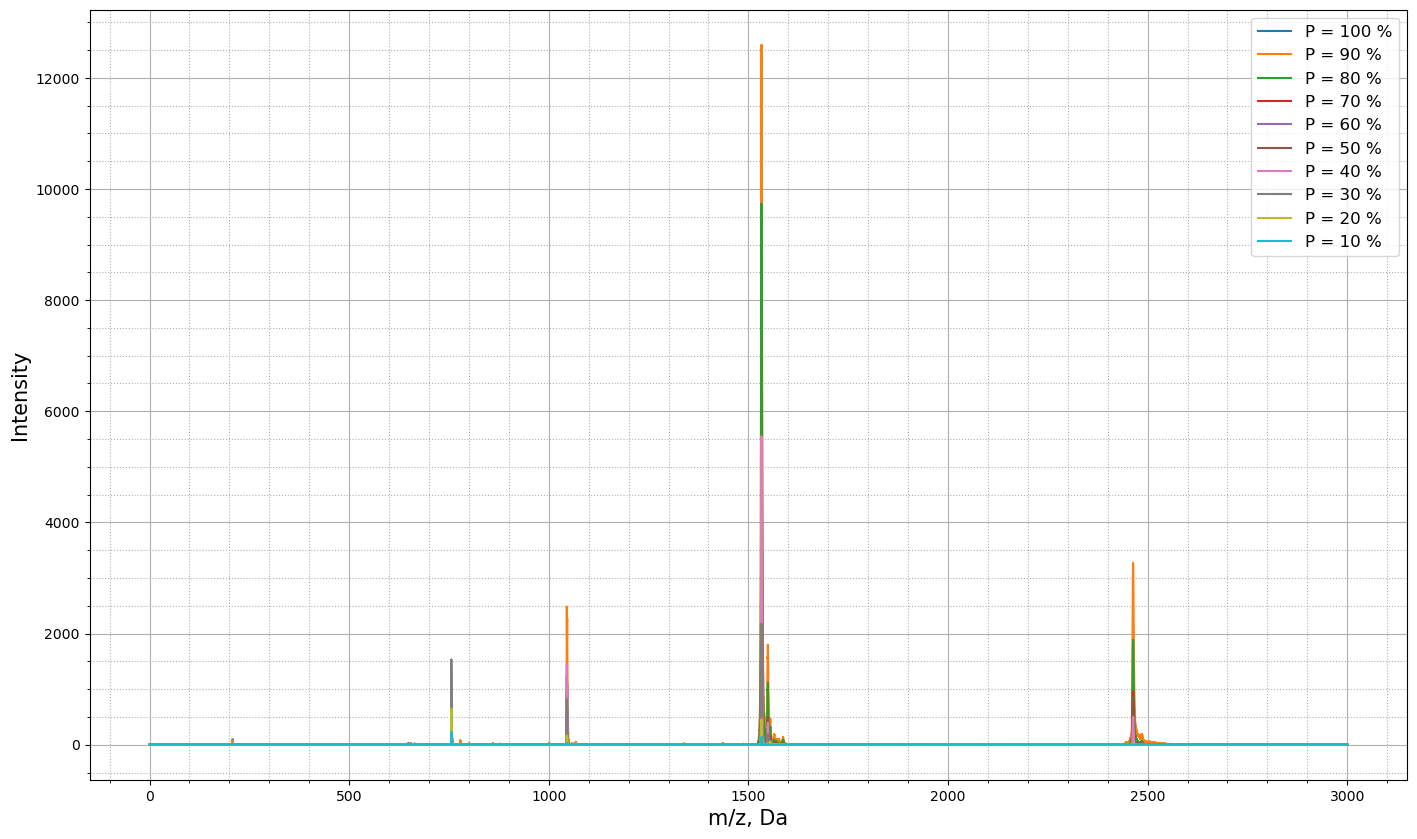
\includegraphics[width=1\linewidth]{Images/linear_power.png}
    \caption{Масс-спектры лунки B22 разной мощности лазера; без рефлектрона}
    \label{Мощность}
\end{figure}

По представленное иллюстрации можно сказать, что:
\begin{itemize}
    \item В целом, с увеличением мощности увеличивается и интенсивность сигнала (однако здесь нельзя установить прямую зависимость, так как полученные спектры - результат сложения нескольких произвольного количества для каждого значения мощности)
    \item Количество пиков на спектре не постоянно, что может свидетельством неравномерном распределении молекул тех или иных белков (или их фрагментов) по всей лунке
\end{itemize}

Проведём теперь измерения указанных характеристик. Полученные зависимости показаны на Рис.\ref{SNR - power}, Рис.\ref{Re - power}, Рис.\ref{Ещё детали} и Рис.\ref{Детали}.

\begin{figure}[h!] 
        \centering
        \minipage{0.5\textwidth}
        \centering
            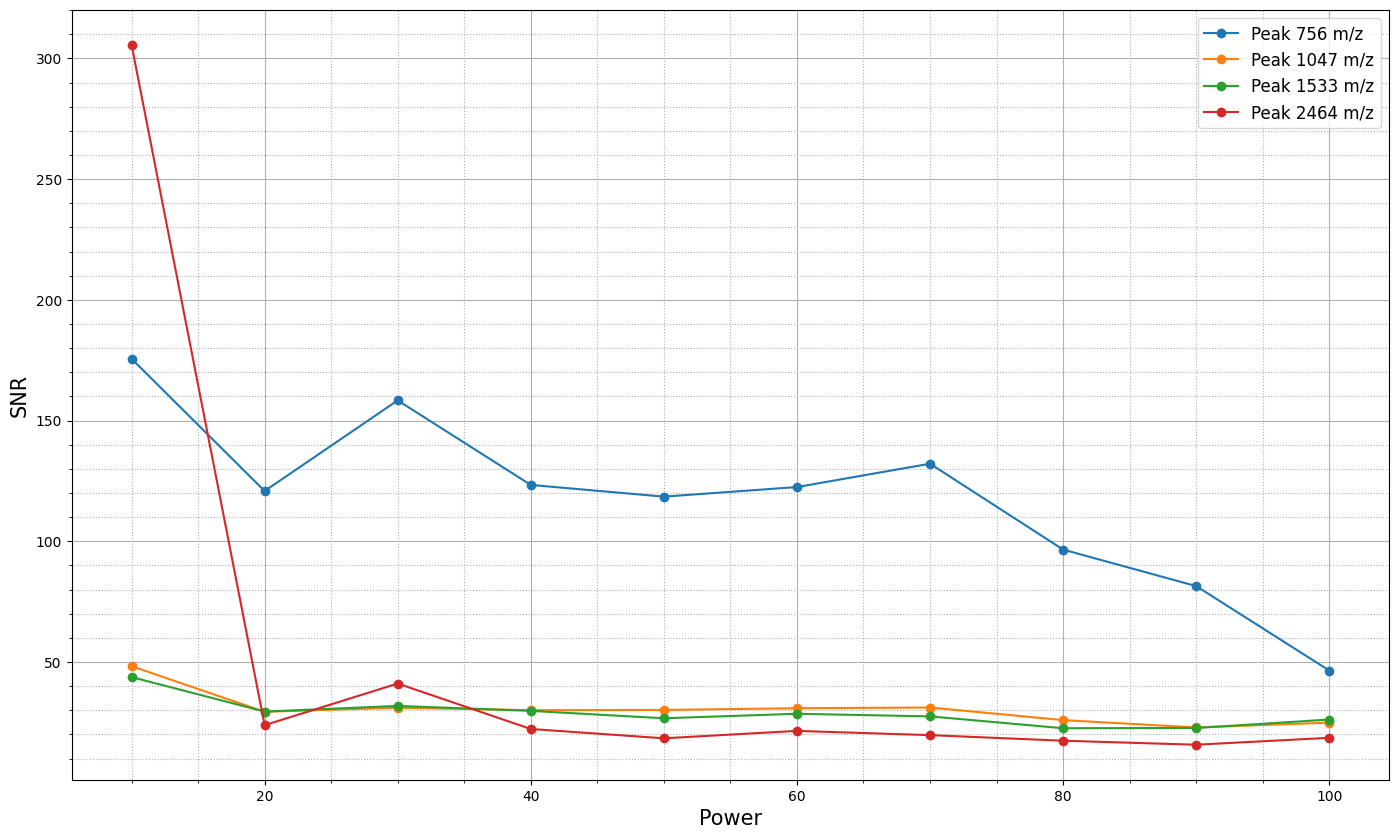
\includegraphics[width=0.9\linewidth]{Images/SNR_power_linear.png}
                 \caption{S/N от разной мощности лазера}
                 \label{SNR - power}
        \endminipage\hfill
        \minipage{0.5\textwidth}
        \centering
             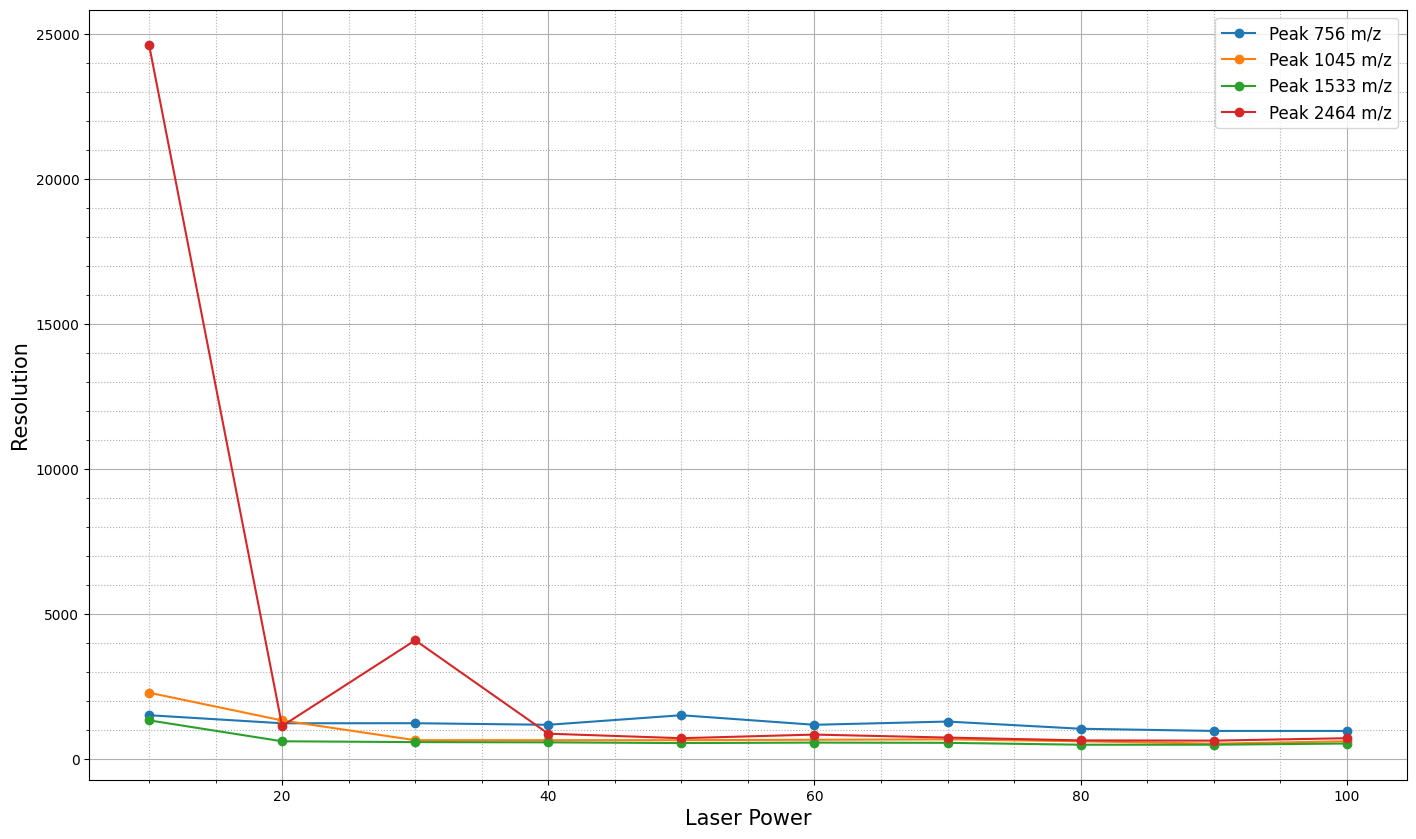
\includegraphics[width=0.9\linewidth]{Images/Resolution_power_linear.png}
                 \caption{Resolution от разной мощности лазера}
                 \label{Re - power}
        \endminipage
\end{figure}

\begin{figure}[h!] 
        \centering
        \minipage{0.5\textwidth}
        \centering
            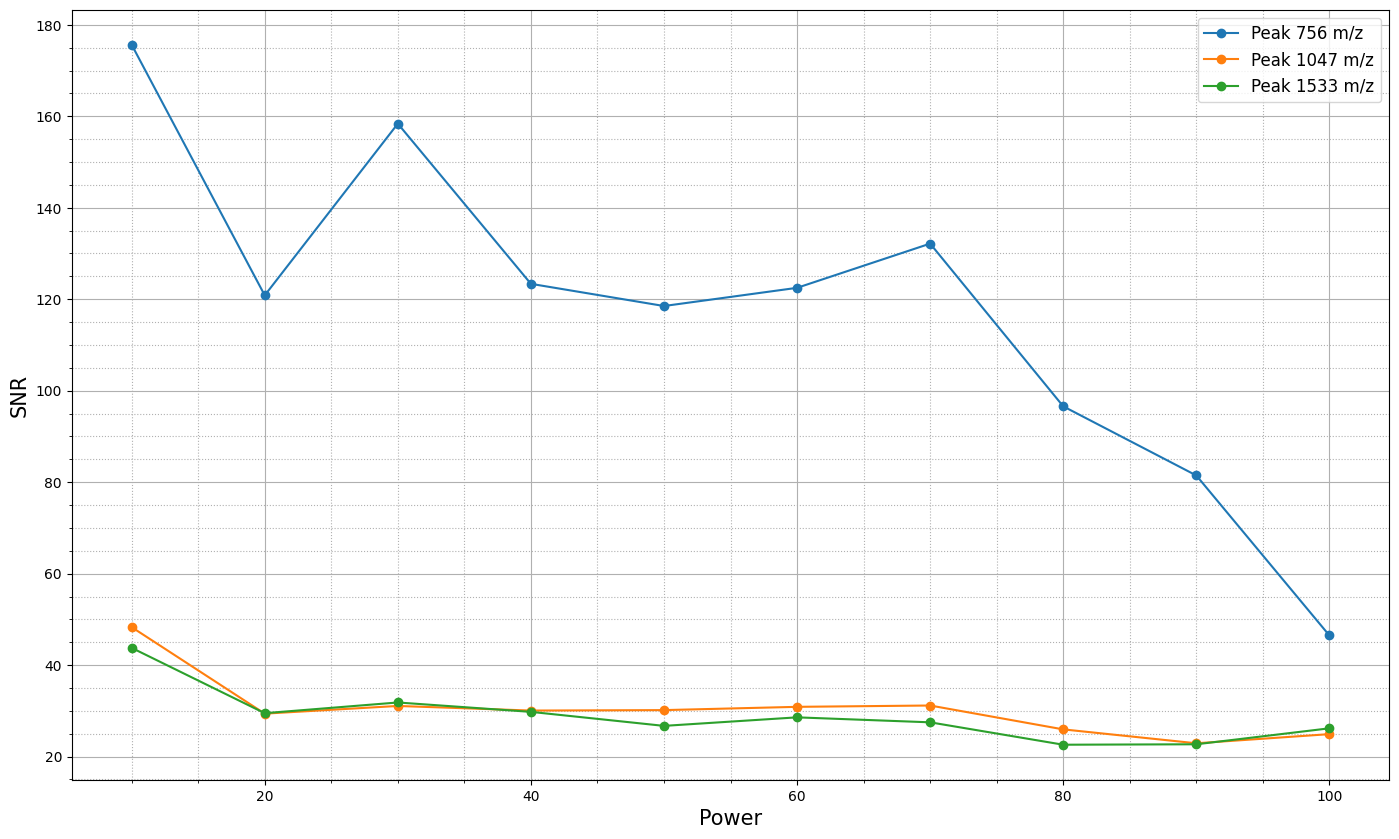
\includegraphics[width=0.9\linewidth]{Images/SNR_power_linear_details.png}
                 \caption{S/N от разной мощности лазера: детали}
                 \label{Ещё детали}
        \endminipage\hfill
        \minipage{0.5\textwidth}
        \centering
             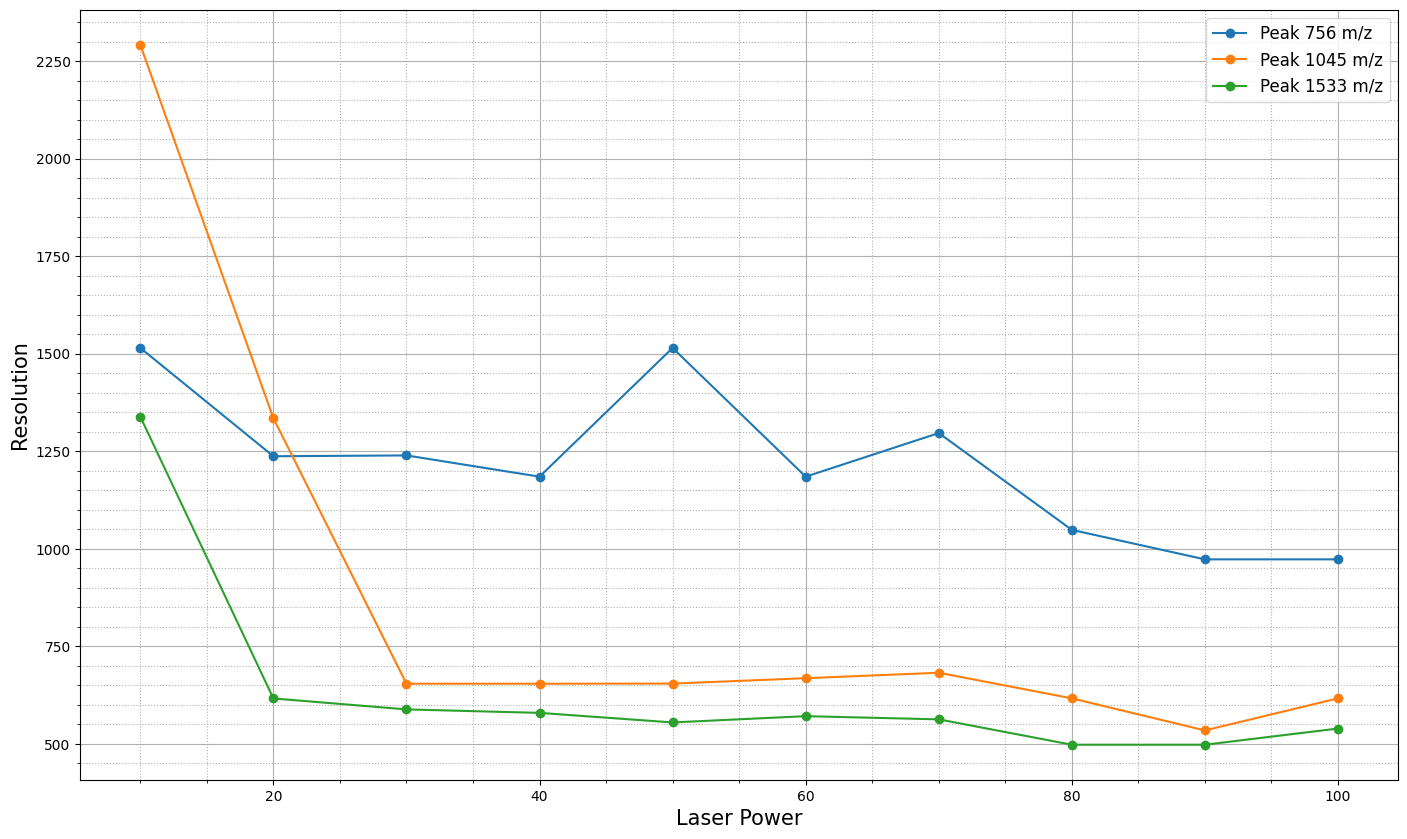
\includegraphics[width=0.9\linewidth]{Images/Resolution_power_linear_details.png}
                 \caption{Resolution от разной мощности лазера: детали}
                 \label{Детали}
        \endminipage
\end{figure}

По представленным графикам можно заключить следующее:
\begin{itemize}
    \item Касательно SNR (Signal to Noise Ratio), можно отметить общую тенденцию к уменьшению с увеличением мощности лазера. Причиной тому может являться увеличивающийся вместе с мощностью шум. Что логично, ведь лазер большей мощности приводит к ионизации большего количества молекул и к деструкции некоторых. Следовательно, SNR постепенно уменьшается. Однако, увеличение мощности также приводило к росту интенсивности пиков - это видно на двух пиках для $756 \; Da$, а также на практически ровных участках у $1047 \; Da$ и $1533 \; Da$. 
    \item Для Resolution можно отметить общую тенденцию на спад, что легко объяснить: при большей мощности лазера в факеле появляется больший разброс частиц по энергии и по координате, следовательно, происходит уширение пиков, т.е. уменьшение разрешения. При малой мощности лазера разрешение пика может ухудшаться из-за недостаточного количества ионов (недостаточная статистика). Стоит отметить выбивающуюся из общего массива линию для $2464 \; Da$. Столь высокое начальное значение можно объяснить тем, что при мощности в $10 \%$ данного пика вообще почти не наблюдалось в общей картине масс-спектра (объясняется или малой концентрацией этого вещества, или недостаточной мощностью и плохой способностью ACTH ионизироваться) 
\end{itemize}

\subsubsection{Определение зависимости аналитических характеристик метода от времени включения ускоряющего потенциала PIE}
\begin{figure}[h!]
\centering
    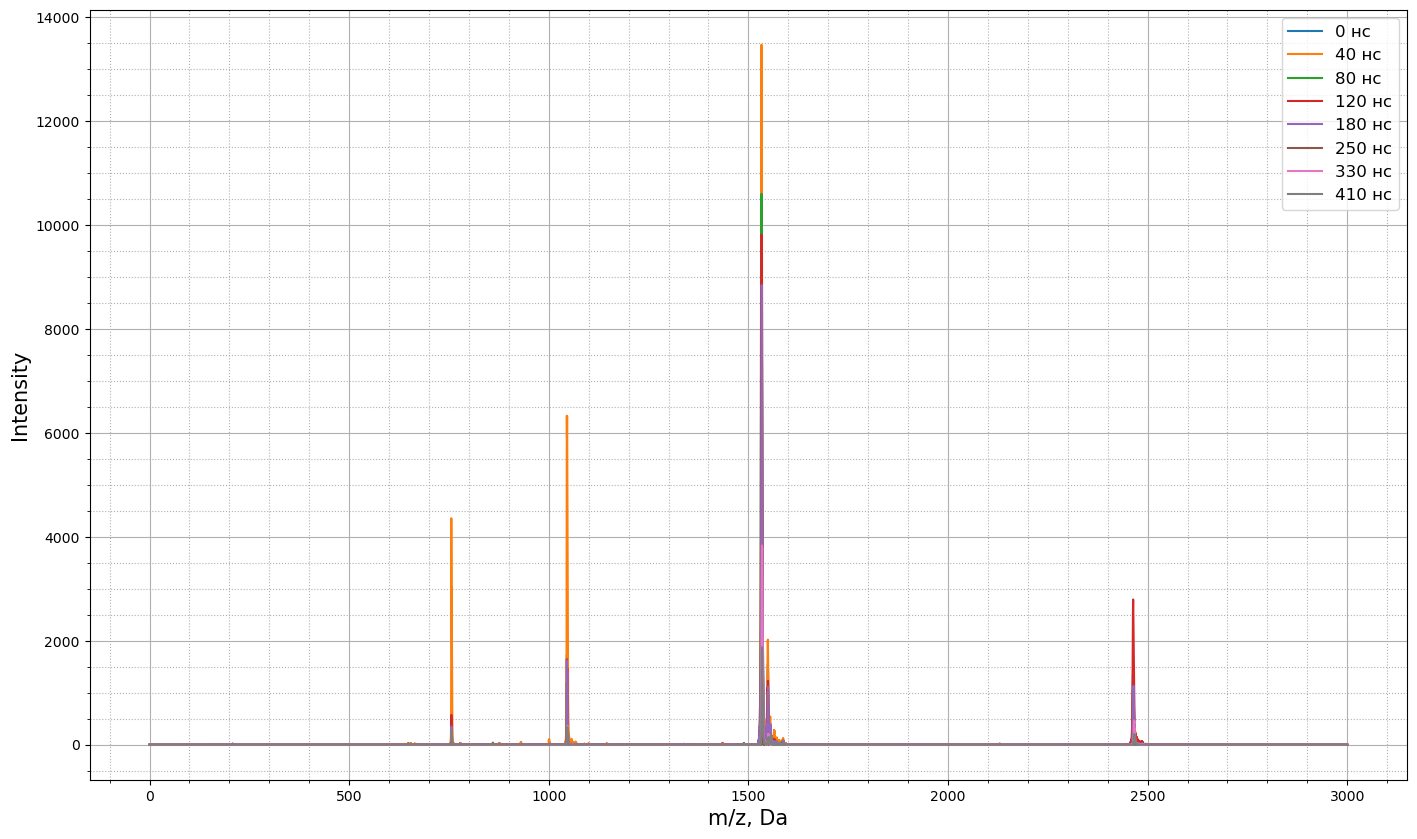
\includegraphics[width=0.7\linewidth]{Images/PIE.png}
    \caption{Масс-спектры лунки B22 разного PIE; без рефлектрона}
    \label{Общее}
\end{figure}
\par Зафиксируем deflection равным 600 и будем изменять время включения ускоряющего потенциала (PIE). Из-за теплового разброса ионы обладают разной начальной скоростью. Подобрав оптимальное PIE, ионы заданной массы будут достигать детектора в один момент времени.
\begin{figure}[h!] 
        \centering
        \minipage{0.5\textwidth}
        \centering
            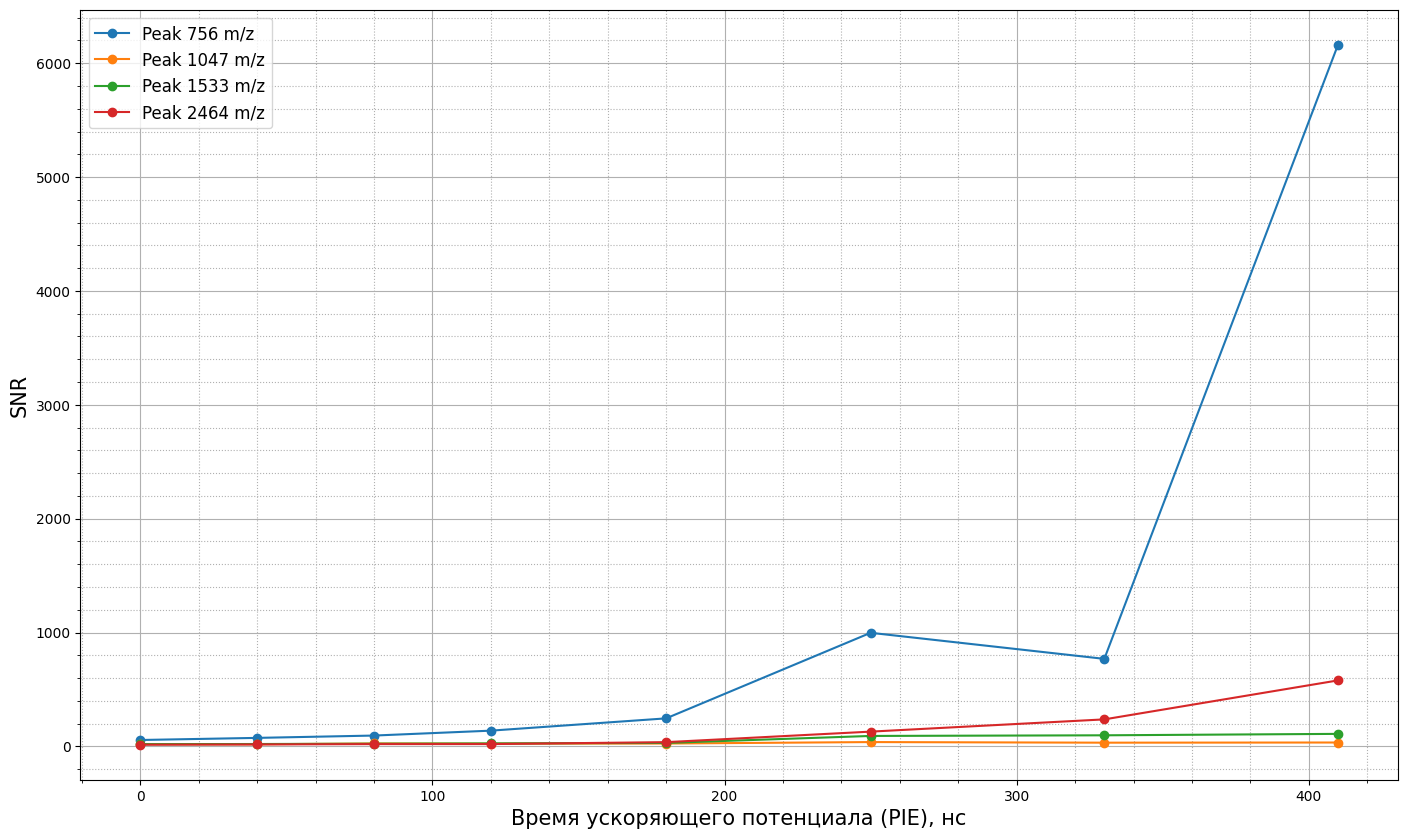
\includegraphics[width=0.9\linewidth]{Images/SN(PIE).png}
                 \caption{S/N от PIE}
                 \label{SNR - PIE}
        \endminipage\hfill
        \minipage{0.5\textwidth}
        \centering
             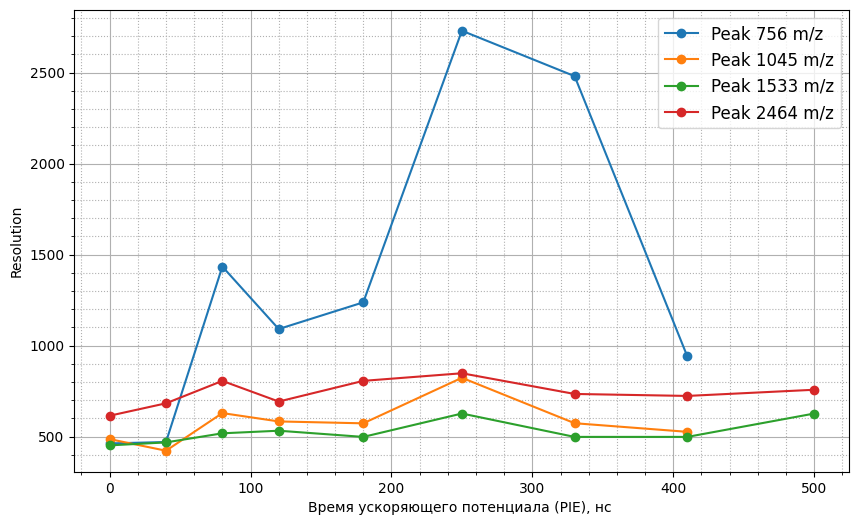
\includegraphics[width=0.9\linewidth]{Images/Res(PIE).png}
                 \caption{Resolution от PIE}
                 \label{Re - PIE}
        \endminipage
        
\end{figure}

\begin{figure}[h!]
\centering
    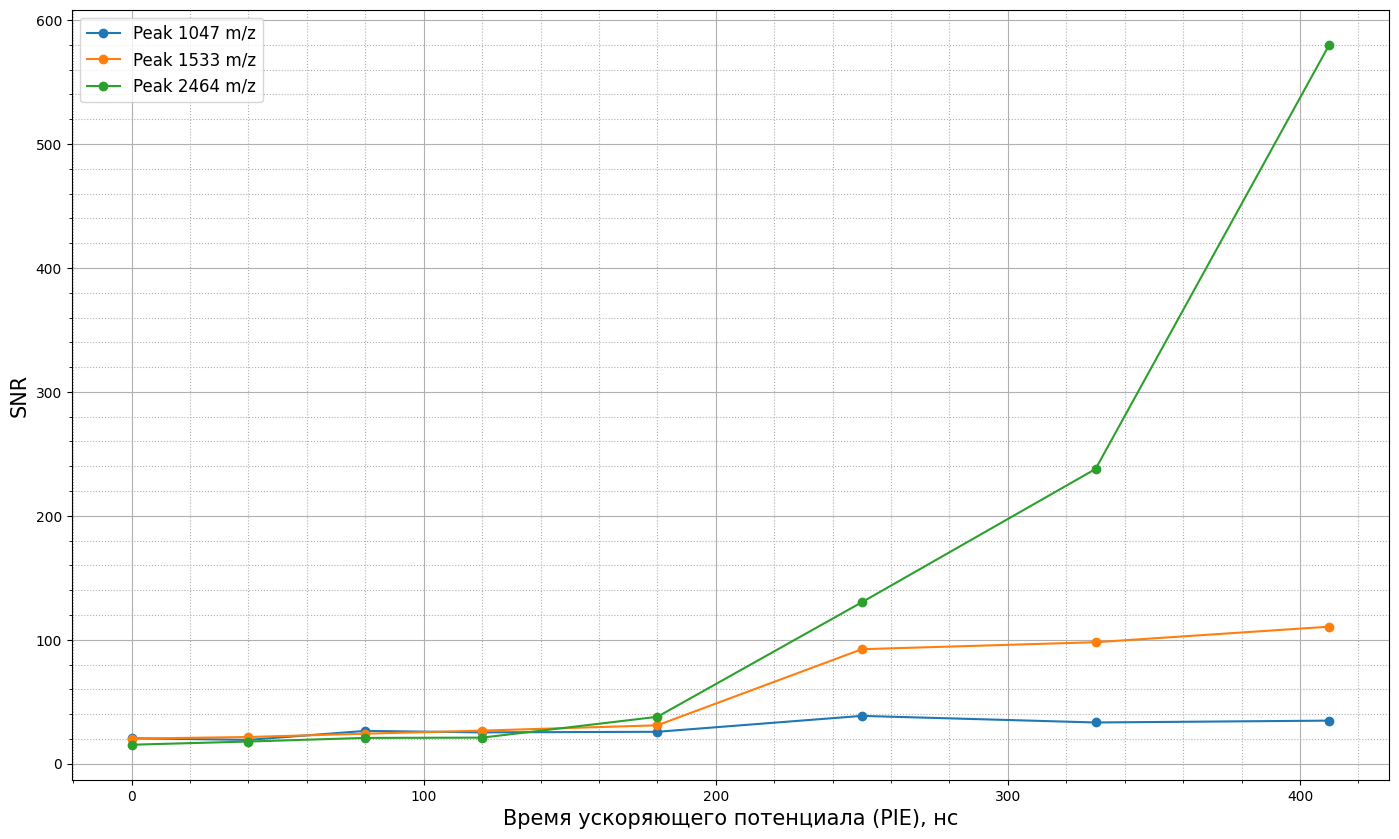
\includegraphics[width=0.6\linewidth]{Images/SNR(PIE) details.png}
    \caption{S/N от PIE: детали}
    \label{Детали 3}
\end{figure}

\par Из полученного графика (Рис. \ref{Re - PIE}) видно, что оптимальное время задержки зависит от m/z для нашей смеси находится в районе 250 нс, при котором значения разрешения достигает максимума. 

На графике S/N Рис. \ref{SNR - PIE} и Рис. \ref{Детали 3} можно отметить, что с увеличением времени ускоряющего потенциала наблюдается увеличение SNR.
\newpage
\subsubsection{Определение зависимости аналитических характеристик метода от уровня подавления матрицы (Deflection)}\; 
\par Проведём измерения при разных значениях Deflection: от $0 \; Da$ до $1200 \; Da$. Для визуального сравнения совместим все графики на одном (Рис.\ref{Deflection})
\begin{figure}[h!]
\centering
    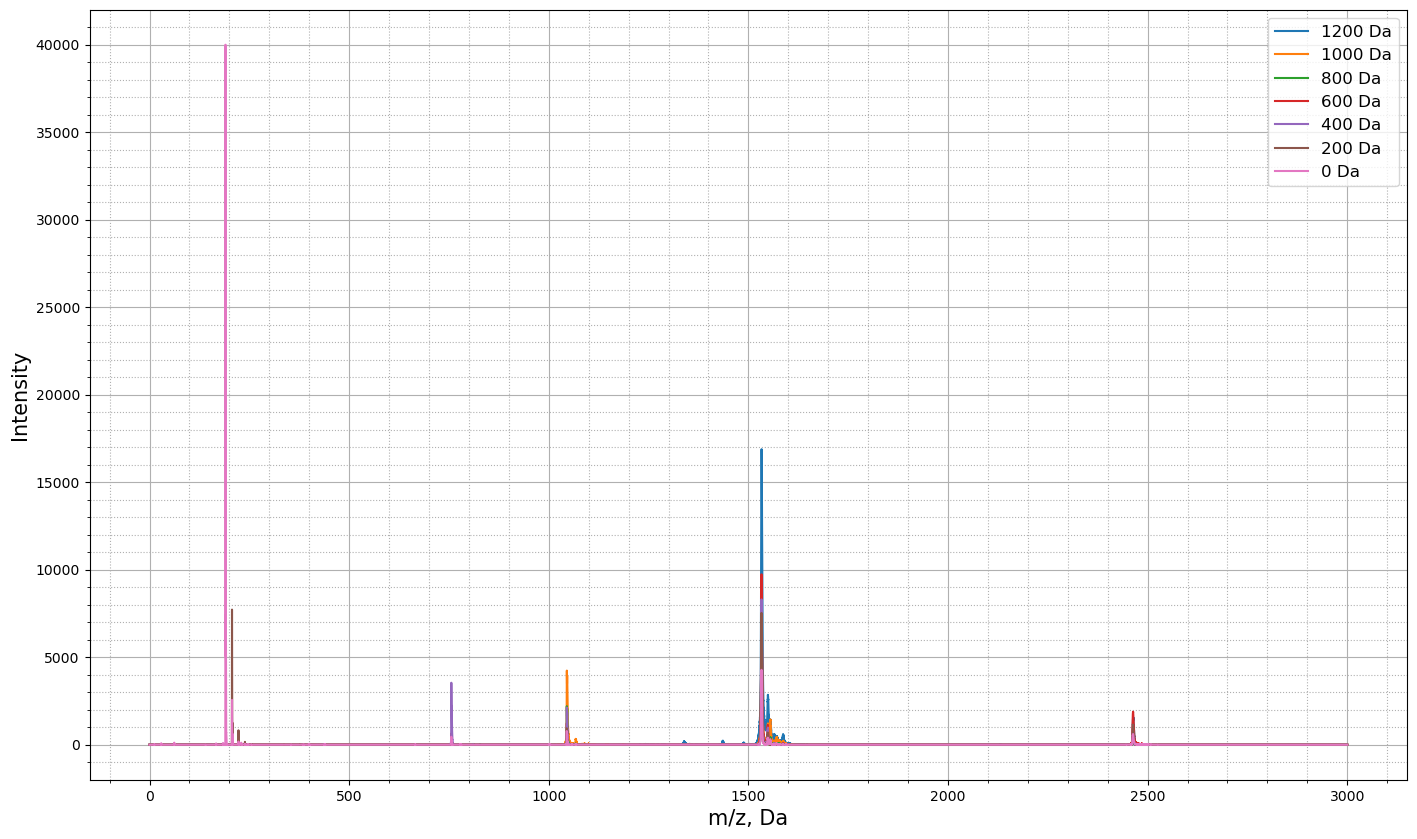
\includegraphics[width=1\linewidth]{Images/Deflection.png}
    \caption{Масс-спектры лунки B22 разного уровня подавления матрицы; без рефлектрона}
    \label{Deflection}
\end{figure}

На приведённом графике видно, что параметр Deflection влияет на количество наблюдаемых пиков. Чем он выше, тем меньшее количество пиков мы можем обнаружить. Это необходимо, например, для того чтобы аминокислотные фрагменты белков не "захламляли" спектр лишними пиками. 

Проведём теперь сравнение выделяемых нами характеристик при разных значениях Deflection: Рис.\ref{SNR - deflection} и Рис.\ref{Re - deflection}.

\begin{figure}[h!] 
        \centering
        \minipage{0.5\textwidth}
        \centering
            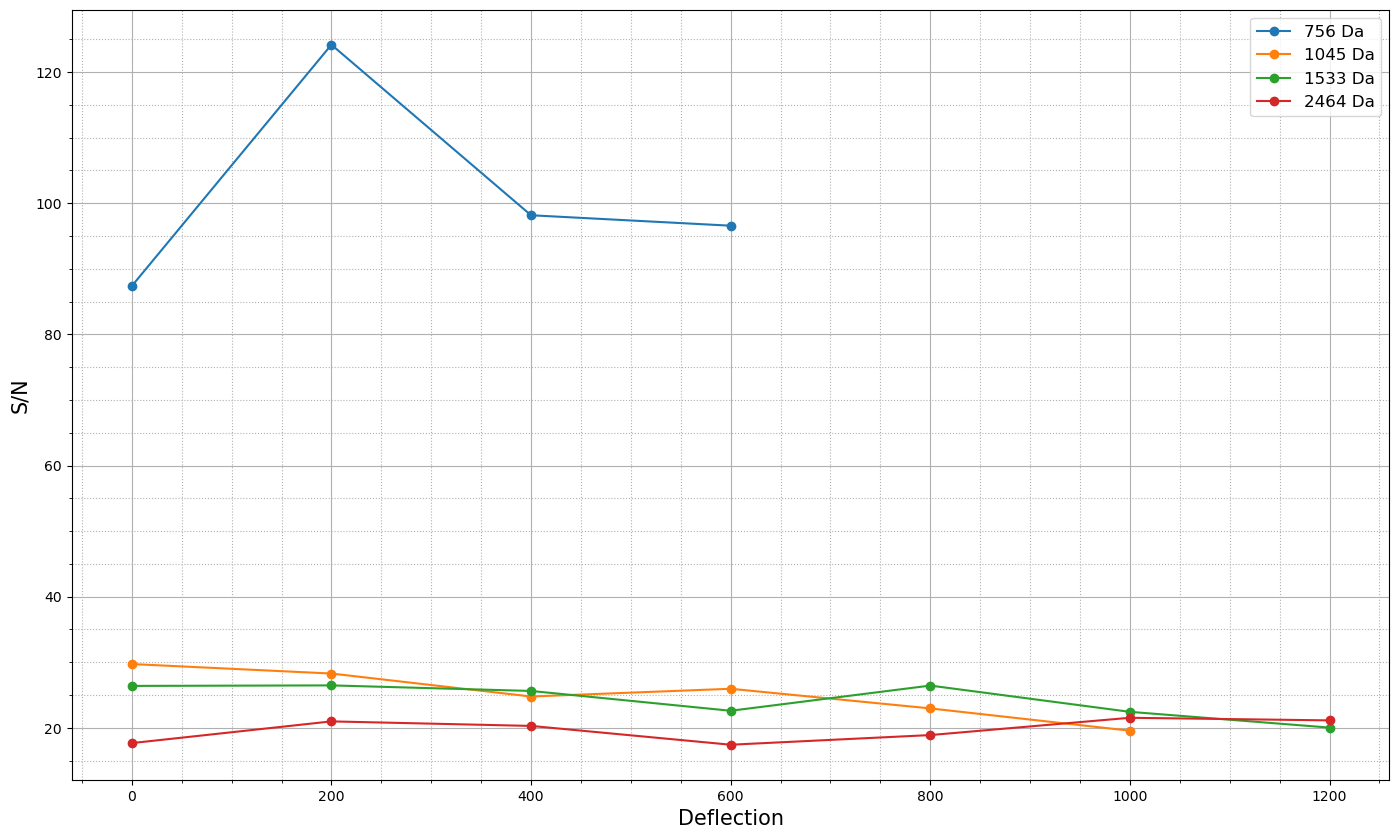
\includegraphics[width=0.9\linewidth]{Images/SNR_deflection.png}
                 \caption{S/N при разном Defletion}
                 \label{SNR - deflection}
        \endminipage\hfill
        \minipage{0.5\textwidth}
        \centering
             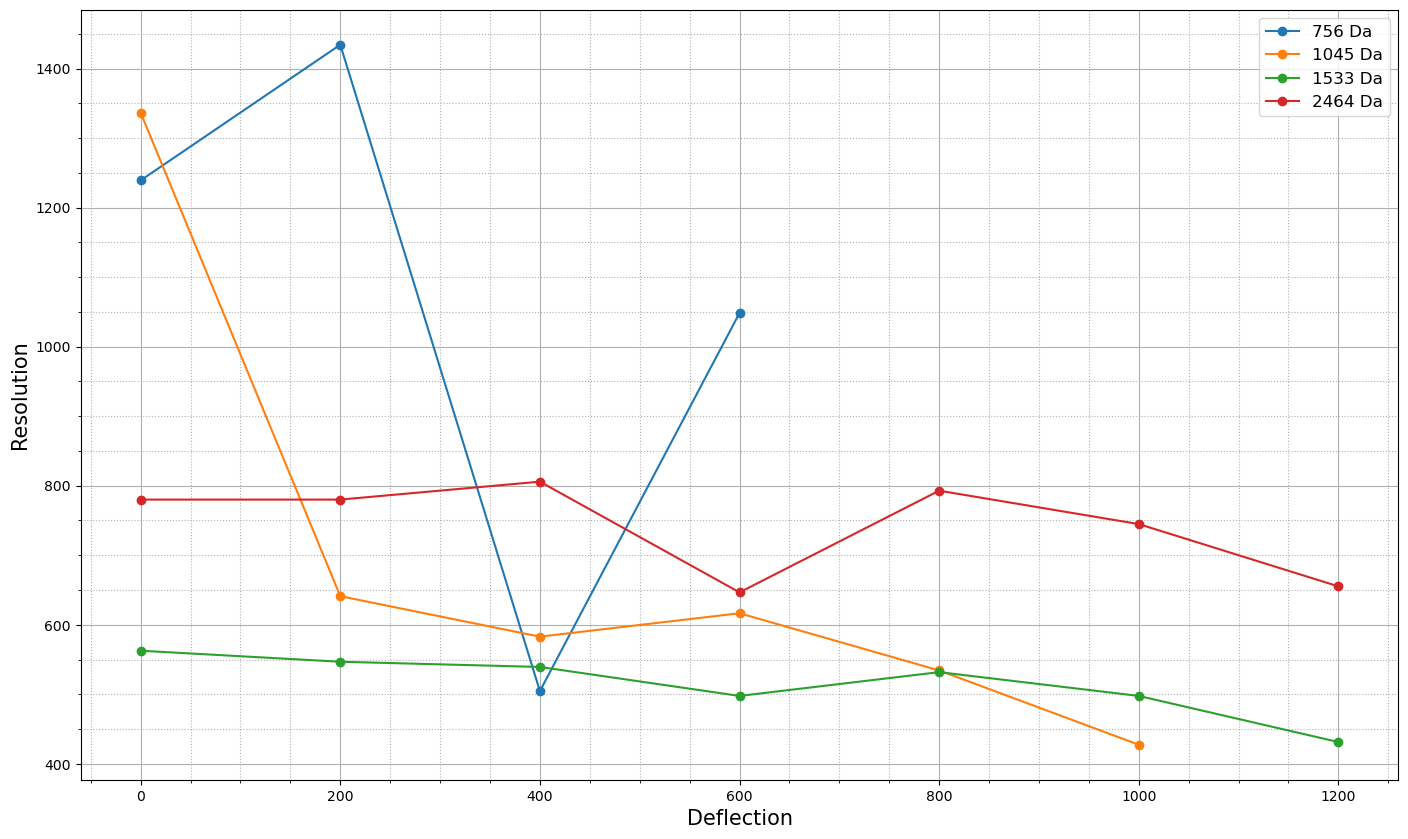
\includegraphics[width=0.9\linewidth]{Images/Re_deflection.png}
                 \caption{Resolution при разном Defletion}
                 \label{Re - deflection}
        \endminipage
\end{figure}


На основании этих графиков можно заметить следующее:
\begin{itemize}
    \item При соответствующем уровне Deflection значения характеристик не определены, потому что при данных значениях сами пики перестают наблюдаться.
    \item SNR, можно сказать, практически не зависит от Deflection, за исключением пика $1045 \; Da$, у которого наблюдается уменьшение SNR с ростом Deflection. Причины этого до конца не ясны.
    \item График Resolution для каждого пика зависит по-разному. Максимумы на графики - соответствуют максимальному разрешению пика и соответствующему уровню подавления матрицы.
\end{itemize}

\subsection{Исследование масс-спектрометрии с рефлектроном}
\subsubsection{Определение зависимости аналитических характеристик метода от мощности лазера}\;

\par Теперь рассмотрим масс-спектр той же лунки B22, но теперь в режиме использования рефлектрона, позволяющего фокусировать ионы.
\begin{figure}[h!]
\centering
    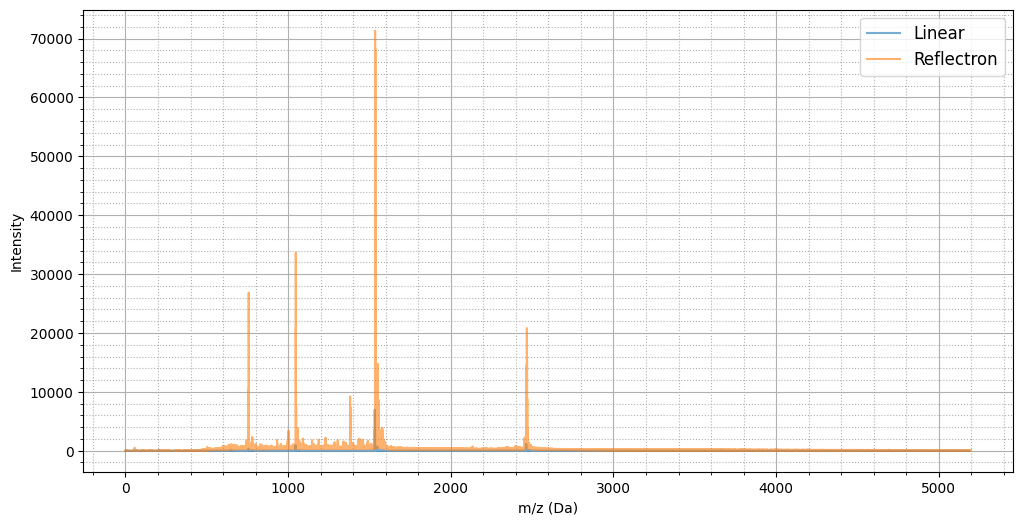
\includegraphics[width=1\linewidth]{Images/linear vs reflectron.png}
    \caption{Масс-спектры лунки B22 c 100\% мощностью лазера без и с использованием рефлектрона}
    \label{lin vs ref}
\end{figure}
\par На объединённом масс-спектре (Рис. \ref{lin vs ref}) видно, как с использованием рефлектрона заметно вырастает интенсивность наших характерных пиков. Причём с увеличением m/z рост замедляется.
\par Аналогично случаю без использования рефлектрона рассмотрим зависимость SNR и Resolution от мощности лазерного излучения (Рис. \ref{SN - reflecton}, \ref{Re - reflecton}). Для разрешения так же характерно уменьшение с увеличением мощности. А вот для SNR становится видно увеличение с ростом мощности и выход на плато для большинства пиков. Возможно, при малой интенсивности лазера шум не связан с характеристиками пептидов, а обусловлен только параметрами установки. В то время как на высоких мощностях лазера молекулы могут фрагментироваться, что приводит к уширению пиков и снижению разрешения.
\begin{figure}[h!] 
        \centering
        \minipage{0.5\textwidth}
        \centering
            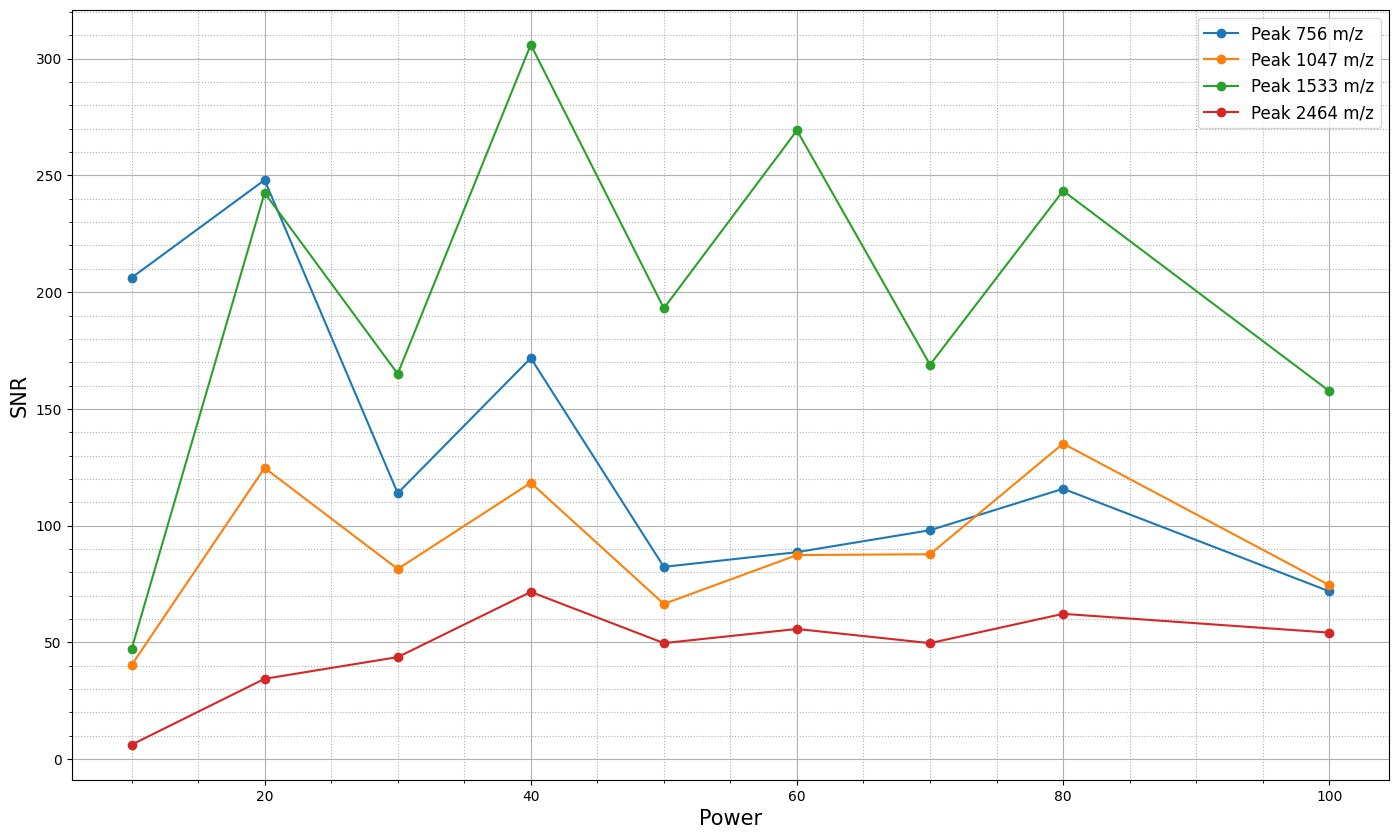
\includegraphics[width=0.9\linewidth]{Images/SN(reflectron).jpg}
                 \caption{S/N от разной мощности лазера с использованием рефлектрона}
                 \label{SN - reflecton}
        \endminipage\hfill
        \minipage{0.5\textwidth}
        \centering
             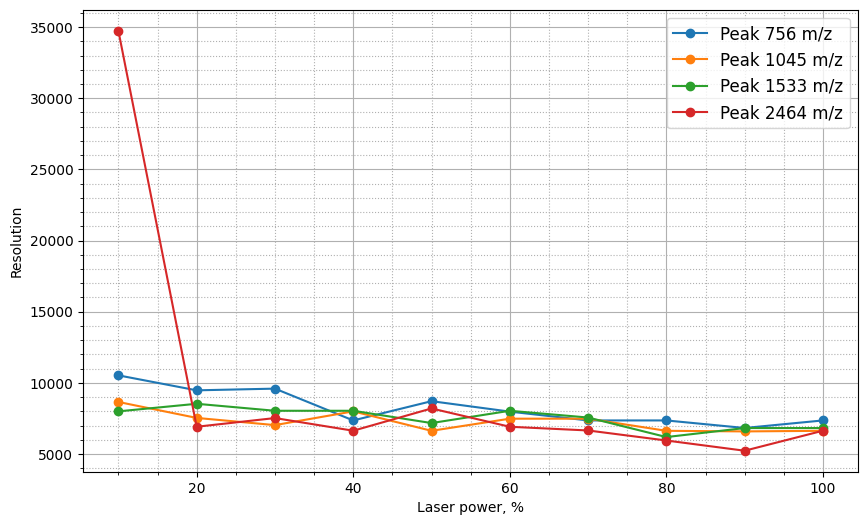
\includegraphics[width=0.9\linewidth]{Images/Res(reflecton).png}
                 \caption{Resolution от разной мощности лазера с использованием рефлектрона}
                 \label{Re - reflecton}
        \endminipage
\end{figure}
\par Сравним характеристики для метода с использованием рефлектрона и без (Рис. \ref{Re - reflecton vs linear}). Благодаря выравниванию частиц по энергиям в отражательном методе однозначно заметно увеличение разрешения в несколько раз.

\begin{figure}[h!]
\centering
    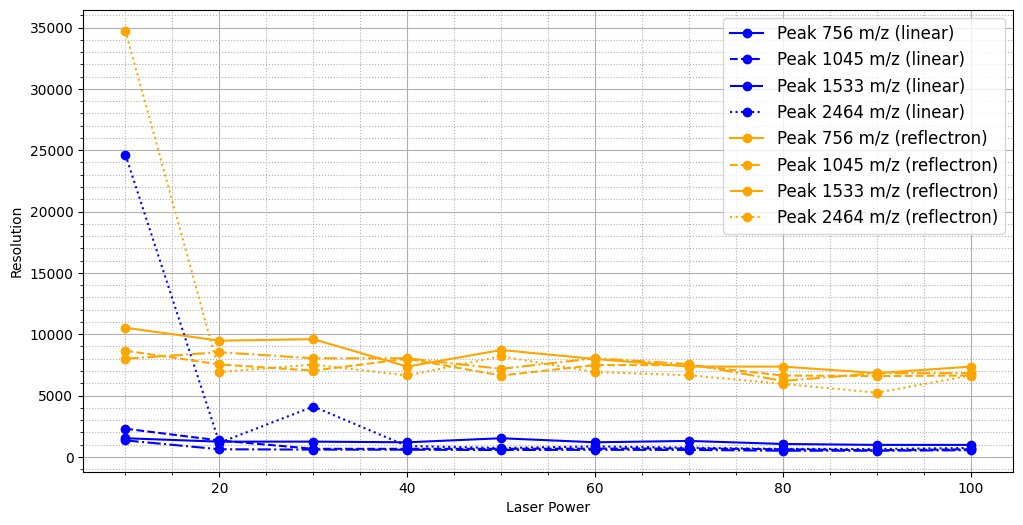
\includegraphics[width=1\linewidth]{Images/Pes(power) lin-ref.png}
    \caption{Resolution от разной мощности лазера без и с использованием рефлектрона}
    \label{Re - reflecton vs linear}
\end{figure}

\subsection{Примеры масс-спектров других белков с рефлектроном и без}\;
\par Для сравнения снимем масс-спектры других лунок (с брадикинином и лизоцимом). Кроме того для брадикинина будем использовать рефлектрон, а для лизоцима - нет. Результаты представлены на Рис.\ref{Брадикинин} и Рис.\ref{Лизоцим}. 

\begin{figure}[h!] 
        \centering
        \minipage{0.5\textwidth}
        \centering
            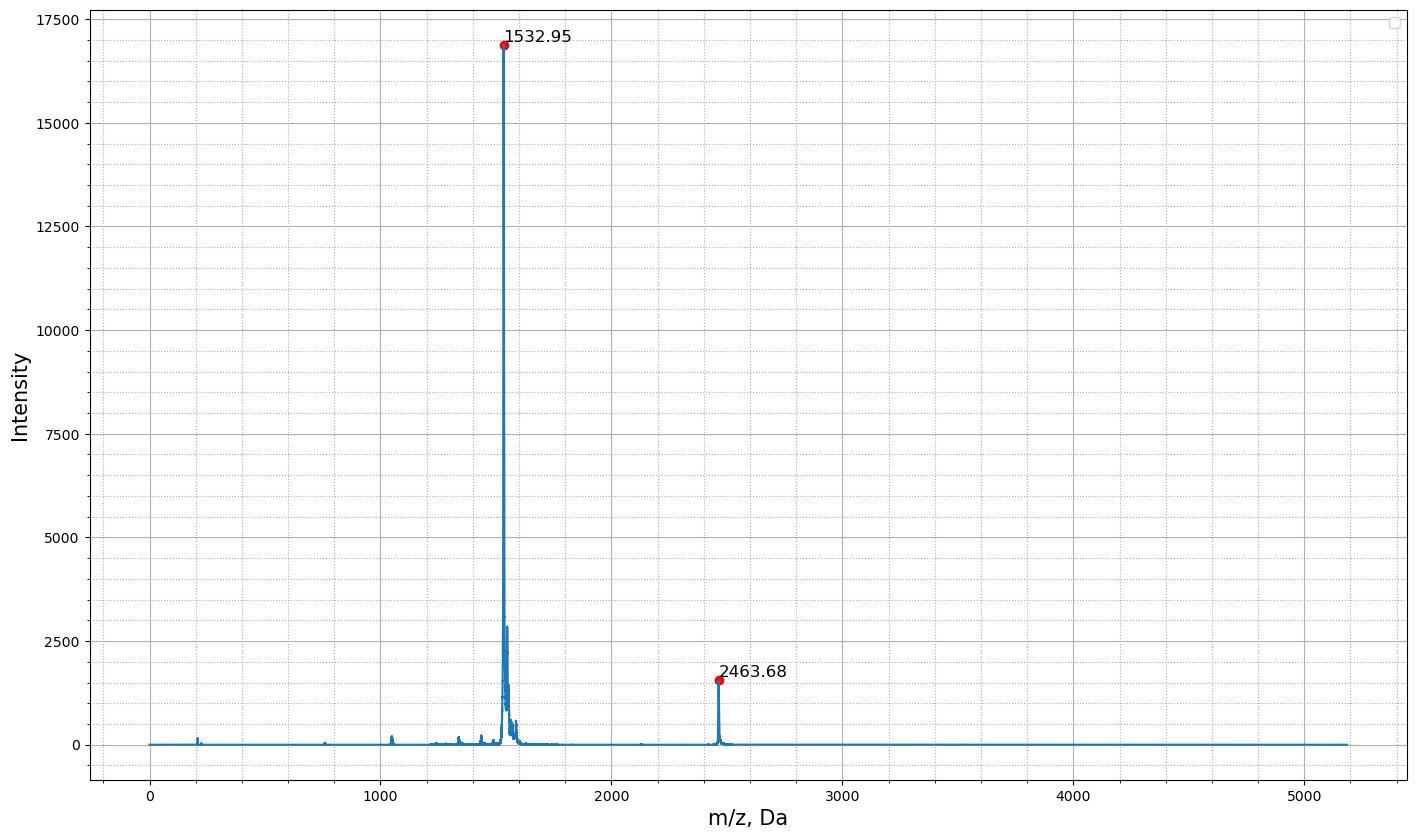
\includegraphics[width=0.9\linewidth]{Images/e23_lisocim.png}
                 \caption{Масс-спектр лизоцима; без рефлектрона}
                 \label{Лизоцим}
        \endminipage\hfill
        \minipage{0.5\textwidth}
        \centering
             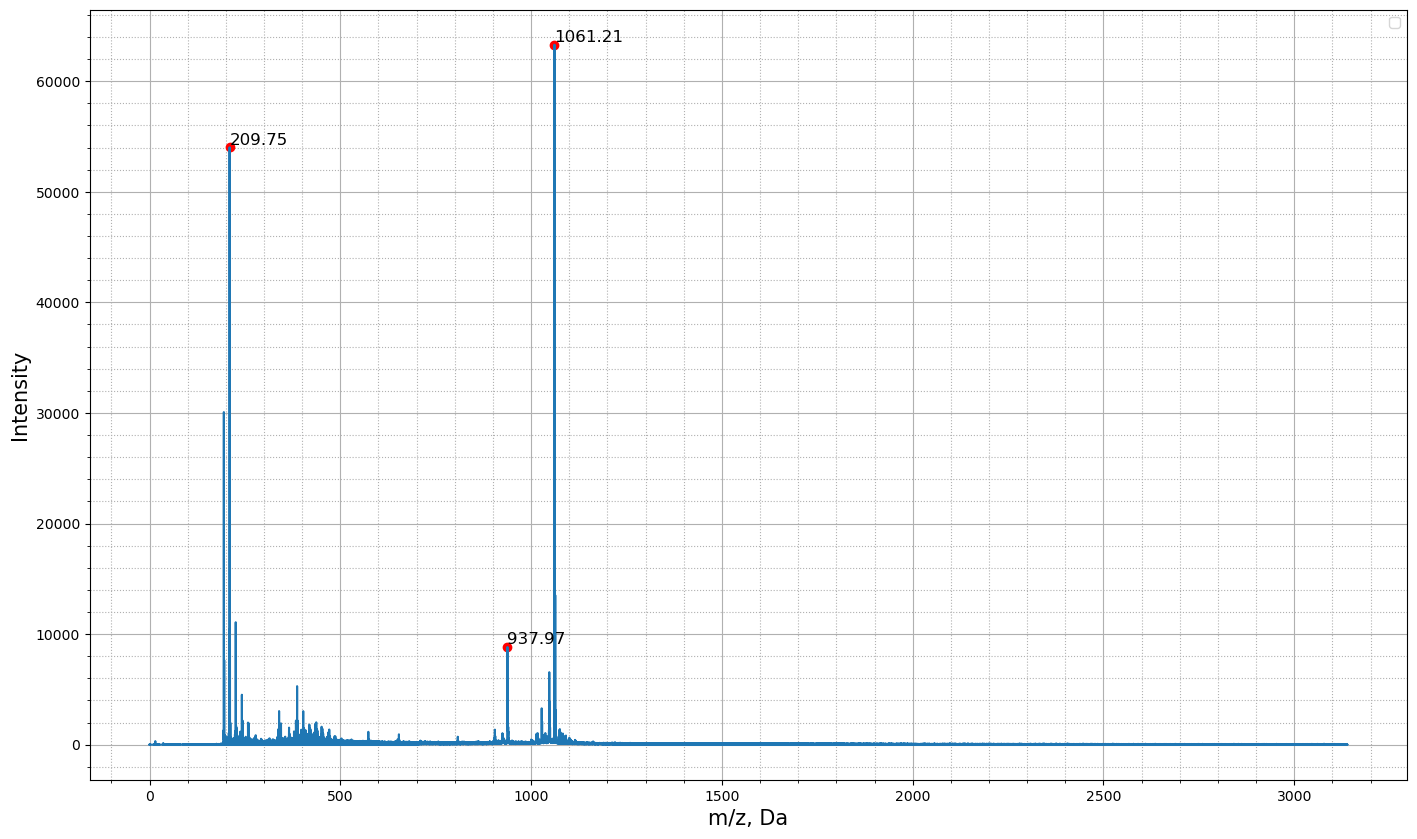
\includegraphics[width=0.9\linewidth]{Images/f21_bradikinin.png}
                 \caption{Масс-спектр брадикинина; с рефлектроном}
                 \label{Брадикинин}
        \endminipage
\end{figure}

Проводя идентификацию пиков, получим:
\begin{itemize}
    \item $1061 \; Da$ - соответствует пику брадикинина, чья масса равна 1060 Да.
    \item Все остальные пики, вероятно, представляют собой фрагменты брадикинина и лизоцима. Определить какие именно не удалось.
\end{itemize}
\newpage
\section{Выводы}
\begin{itemize}
    \item На масс-спектрах были определены 4 основных пика, которым соответствуют следующие пептиды:
    \begin{table}[h!]
    \centering
    \begin{tabular}{|l|l|}
    \hline
    m/z, Да & Пептид           \\ \hline
    $756\pm1$     & Bradykinin (1–7) \\ \hline
    $1046\pm1$    & Angiotensin II   \\ \hline
    $1533\pm1$    & P14R             \\ \hline
    $2464\pm1$    & ACTH (18–39)     \\ \hline
    \end{tabular}
    \end{table}
    \item Использование рефлектрона позволило увеличить разрешающую способность в несколько раз за счёт компенсации разброса кинетической энергии ионов.
    \item Также в ходже работы были выявлены зависимости основных характеристик (разрешения и отношения сигнал/шум) масс-спектрометра от настроек измерений. В частности:
    \begin{itemize}
        \item Linear: SNR уменьшается с увеличением мощности спектрометра;
        \item Linear: Resolution уменьшается с увеличением мощности;
        \item Linear: SNR растёт с ростом PIE;
        \item Linear: зависимость Resolution от PIE позволяет определить при каком значении настройки наблюдается максимальное разрешение;
        \item Linear: SNR практически не зависит от Deflection;
        \item Linear: зависимость Resolution от Deflection позволяет определить при каком значении настройки наблюдается максимальное разрешение;
        \item Reflectron: SNR растёт с ростом мощности;
        \item Reflectron: Resolution уменьшается с ростом мощности.
    \end{itemize}
    \item Кроме того, была продемонстрирована возможность детектирования с помощью масс-спектрометра как полноценных белков, так и их фрагментов.
\end{itemize}
\end{document}
